\documentclass[12pt]{article}
\usepackage{amsmath}
\usepackage{epsfig,psfrag}
\usepackage{natbib}
\usepackage{graphicx}
\usepackage[shortlabels]{enumitem}
\setlength{\textwidth}{6.5in}
\setlength{\textheight}{8.9in}
\setlength{\voffset}{-1in}
\setlength{\oddsidemargin}{0in}
\setlength{\evensidemargin}{0in}

%biblography of JFM Style
\bibliographystyle{jfm}

%Some mathematical Definitions
\def\o{\over}
\def\p{\partial}
\def\be{\begin{eqnarray}}
\def\ee{\end{eqnarray}}
\def\bes{\begin{subeqnarray}}
\def\ees{\end{subeqnarray}}

\def\f{\frac}
\def\lp{\left(}
\def\rp{\right)}
\def\lb{\left[}
\def\rb{\right]}
\def\lcb{\left\{}
\def\rcb{\right\}}
\def\n{\nabla}
\def\lap{\nabla^2}
\def\z{\zeta}
\def\ep{\epsilon}
\def\l{\lambda}
\def\befi{\begin{figure}}
\def\eefi{\end{figure}}
\def\a{\alpha}
\def\no{\noindent}
\def\h{\hat{}}
\def\bce{\begin{center}}
\def\ece{\end{center}}



\def\d{\text{d}}
\def\vep{\varepsilon}
\def\ep{\epsilon}
\def\la{\langle}
\def\ra{\rangle}
\def\th{\theta}


\title{Percolation}
\author{Ahmad}
%-------------------------------------------------------------------
\begin{document}          
\maketitle


\section{Permeability modification Model}
%
The polymers passing through pores are dragged by the flow. There are
two forces competing when a polymer adheres to the surface of a pore
(1) The drag force on the particle coming from flow, and (2)
ionic/VanderWaals or whatever force that tries to adhere the particles
to the surface. A particle attaches to the surface if the drag force
exerted by the fluid flow around it is smaller than the
VanderWaals/ionic force.

For simplicity, I assume that the force is ionic with a force distance
profile of $F= K/X^2$, where $K$ is a constant and $X$ is the
distance. I assume that polymers have an effective radius of $d_{p}$
and fluid viscosity is $\mu$ and the flow rate is $Q$. This model
states that the particle attaches to the surface when
%%
\begin{align}
    F_{\text{drag}} &\leq F_{\text{ionic}}\\
    6\pi \mu d_{p} \frac{2Q}{\pi R^2} \lp 1- \frac{r^2}{R^2} \rp & \leq \frac{K}{(R-r)^2} \\
    1 - \frac{r^2}{R^2} & \leq \lp \frac{K }{12 \mu  d_{p} Q} \rp \frac{1}{\lp 1 - r/R \rp^2} \\
    1 & \leq \frac{r^2}{R^2} + \alpha \frac{1}{\lp 1-r/R\rp ^2}
\end{align}
%
where $\alpha = K/\lp 12\mu d_pQ \rp$ is a factor that compares the ionic force and viscous
force. Note that it depends on the flux rate. If we define
$x = 1- r/R$ we obtain
%
\begin{align}
    1 &\leq (1-x)^{2} + \frac{\alpha}{x^2} \\
    x^2- x^2(1-x)^{2} &\leq \alpha \\
    x^2 (1- (1-x)^2) & \leq \alpha \\
    x^3(2-x) & \leq \alpha \\
    \text{if } x\ll1 \to x & \leq \lp \frac{\alpha}{2}\rp^{1/3}
\end{align}
%
%
\begin{figure}[h]
  \centering
  \includegraphics[width=4cm]{./Figs/model2.jpg}
  \caption{Flow in the pipe}
\end{figure}
%
As a result the thickness of the adsoption layer is proportional to
$\alpha^{1/3}$. Note that $\alpha$ depends on $1/Q$.  Now, lets find
the flux passing through this adsorption layer (any polymer in this
layer would attach to the surface and therefore I call this layer
adsoption layer)
%
%
\begin{align}
  \text{volume}/\text{time} &= \frac{1}{2} R \alpha ^{1/3} \cdot \frac{Q}{R^{3}} R\a^{1/3} \cdot 2\pi R = \pi Q \a^{2/3}  = \pi \lp \frac{K  }{12 \mu  d_{p}} \rp^{2/3} Q^{1/3} \\
  \text{volume}/\text{time} & \propto {Q^{1/3}} 
\end{align}
%
Now, if we assume that the number of polymers passing through this
area causes clogging, then the change in the total area of the pipe
will be proportional to the flux through adsorption layer

%
\begin{align}
  d (\pi R^2) \propto Q^{1/3} \quad \to \quad R dR \propto Q^{1/3} \label{eq:change-law} \\
  dR \propto \lp \frac{Q}{R^3}\rp^{1/3}
\end{align}
%
which means that the rate of change of the diameter is proportional to
the shear rate to the power of $1/3$. Note that we also know that
$k = \pi R^4/8l^2$, as a result
%
\begin{align}
  dk \propto R^{3} dR \\
  dk \propto R^2 Q^{1/3} \\
  dk \propto Q^{1/3}
\end{align}
%
which means the changes in the permeability is propotional to the
$Q^{1/3}$ passing through the porous media.

\subsection*{Experimental Results}
%
In Shima's paper, we report a figure that shows the evolution of
permeability $k$ per volume of polymer $V_{pol}$ that passes through
the porous media. Basically we are plotting $\Delta k$ versus $Q$
passing through the porous media. The figure and best polynomial fit
is shown blow
%
%
\begin{figure}[h]
  \centering
  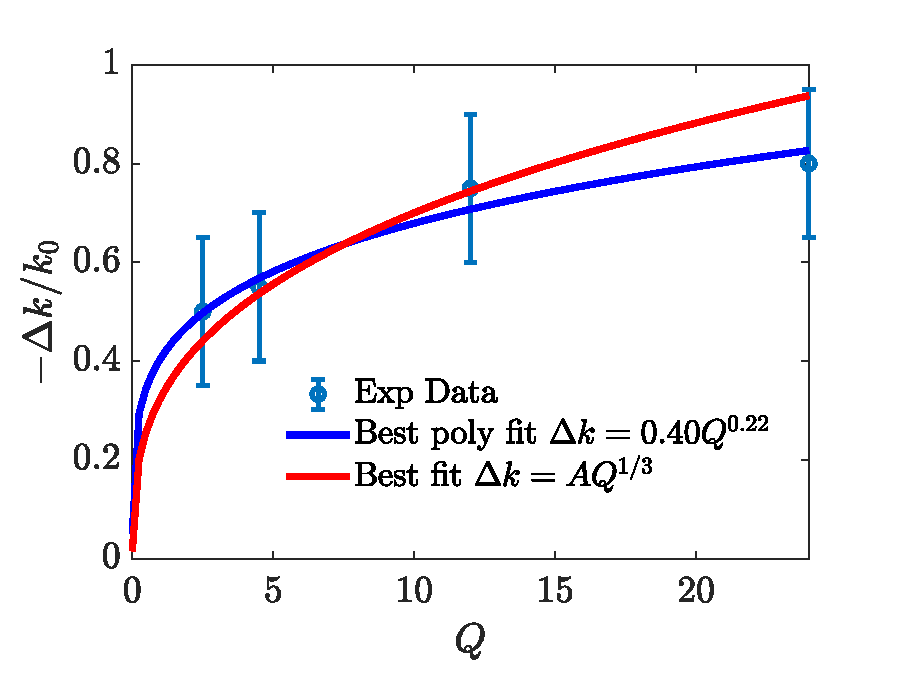
\includegraphics[width=0.55\textwidth]{./Figs/k-evolution.eps}
  \caption{$k$ versus volume of fluid passing through}
\end{figure}



\subsection{Numerical Result}
%
I also ran a numerical simulation in which, I change the diameters
according to \ref{eq:change-law}. The result is as follows
%
\begin{figure}[h]
  \centering
  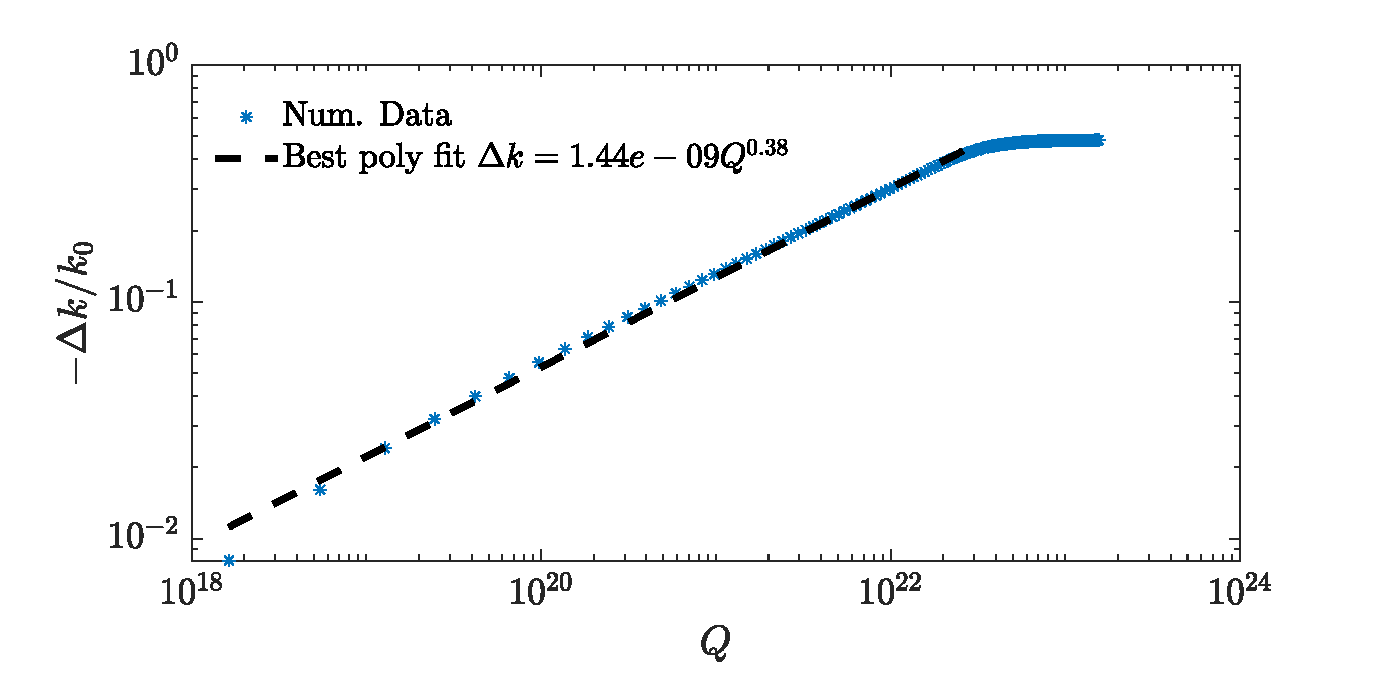
\includegraphics[width=0.55\textwidth]{./Figs/k-evolution-numerics.eps}
  \caption{$k$ versus volume of fluid passing through in numerical
    simulation. Note that the plateau is due to the max limit imposed
    for max reduction in diameter}
\end{figure}

%
\section{General Force term}
%
In this section we assume a general forcing term of type $F_{g} = K/X^n$, and
as a result find the coefficient function. 
%
\begin{align}
    F_{\text{drag}} &\leq  F_g \\
    6\pi \mu d_{p} \frac{2Q}{\pi R^2} \lp 1- \frac{r^2}{R^2} \rp & \leq \frac{K}{(R-r)^{n}} \\
    1 - \frac{r^2}{R^2} & \leq  \frac{K }{12 \mu  d_{p} Q R^{n-2}} \frac{1}{(1-r/R)^{n}}   \\
    1 -\frac{r^2}{R^2} &  \leq   \beta  \frac{1}{(1-r/R)^{n}}
\end{align}
%
where $\beta = {K }/{12 \mu d_{p} Q R^{n-2}} $. If we define $x = 1- r/R$ we obtain
%
\begin{align}
  1 - (1-x)^{2} & \leq \beta \frac{1}{x^{n}} \\
 x^{n+1} \lp 2 - x \rp  &\leq \beta  \\\
  x\ll 1 , \qquad x  & \leq \lp \frac{\beta}{2} \rp^{\frac{1}{n+1} } 
\end{align}
%
%
%
\begin{align}
  \text{volume}/\text{time} &= \frac{1}{2} R \lp \frac{\beta}{2} \rp^{\frac{1}{n+1} }  \cdot \frac{Q}{R^{3}} \lp R \frac{\beta}{2} \rp^{\frac{1}{n+1} } \cdot 2\pi R  \\
  \text{volume}/\text{time} &\propto  Q^{1 - \frac{2}{n+1} } R^{-2\frac{n-2}{n+1} } \\
  \text{volume}/\text{time} &\propto  Q^{\frac{n-1}{n+1} } R^{-2\frac{n-2}{n+1} -1}  R  \\
  \text{volume}/\text{time} &\propto  R  \lp \frac{Q}{R^{3}}   \rp ^{\frac{n-1}{n+1} }
\end{align}
%
%
\begin{align}
  d (\pi R^2) \propto R  \lp \frac{Q}{R^{3}}   \rp ^{\frac{n-1}{n+1} } \quad \to \quad \boxed{dR \propto \lp \frac{Q}{R^{3}}  \rp ^{\frac{n-1}{n+1} }}
\end{align}
%
If $k = \pi R^4/8l^2$, as a result
%
\begin{align}
  dk \propto R^{3} dR \\
  dk \propto R^3 \lp \frac{Q}{R^{3}}  \rp ^{\frac{n-1}{n+1} } \\
  \boxed{dk \propto Q^{\frac{n-1}{n+1}}}
\end{align}
%


\section{Force Consideration}
%
In \cite{montgomery2000analytical}, the authors have summarized
adhesion studies. They show that the interaction between a spherical
molecule and an infinite cylinder, results in the adhesion force of
%
\begin{align}
  F \propto \frac{1}{X^{2}} 
\end{align}
%
where $X$ is the distance between the molecule and the surface. 




\section{Modelling Force}
%
Assuming a tube shape for the pores, the following figure appears
%
\begin{figure}[h]
  \centering
  \includegraphics[width=10cm]{./Figs/polymer-attachment}
  \caption{Polymer attachment to the surface. The polymer is assumed
    to be at distance $x$ to the boundary. We pick the coordinate
    system such that $\hat{z}$ is along the direction of the tube and
    the polymer is on the ${y}$-axis. }
\end{figure}
%
There are 3 different cases:
%
\begin{itemize}
\item \textbf{Constant attraction force}: The polymer is very small compared to the pore radius and is
  very close to the surface such that it does not feel the
  curvature. For particle, the pore is like a flat infintie plate that
  is atttacting the particle. If the attraction force is due to
  columb, then the attracting force is independen of distance and has
  a constant value.

\item If the particle feels the attraction force between an infinite
  cylinder with radius $R$ and a point particle with charge $q$ at
  distance $x$ from the edge can be calculated as 
%
  \begin{align}
    \text{symmetry } F_{x}= F_{z} = 0, \qquad F_y = \int_{-\infty}^{\infty} \int_0^{2 \pi} \frac{R\sin\th - R + x}{\lp R^{2} -2 R (R-x) \sin\th + z^2\rp^{3/2}} q \lambda R d\th   
  \end{align}
  %
  Using mathematica, so far, I was unable to find the leading power of
  force in terms of $x$.
   
\end{itemize}



\section{Lennard-Jones Force}
%
\begin{align}
    F_{\text{drag}} &\leq F_{LJ}\\
  6\pi \mu d_{p} \frac{2Q}{\pi R^2} \lp 1- \frac{r^2}{R^2} \rp & \leq 48\ep \lb \frac{\sigma^{12}}{(R-r)^{13}} - \frac{\sigma^{6}}{(R-r)^{7}}  \rb \\
  6\pi \mu d_{p} \frac{2Q}{\pi R^2} \lp 1- \frac{r^2}{R^2} \rp & \leq 48\ep \lb \frac{(\sigma/R)^{12}}{(1-r/R)^{13}} - \frac{(\sigma/R)^{6}}{(1-r/R)^{7}}  \rb \\
  6\pi \mu d_{p} \frac{2Q}{\pi R^2} \lp 1- (1-x)^2\rp & \leq 48\ep \lb \frac{(\sigma/R)^{12}}{x^{13}} - \frac{(\sigma/R)^{6}}{x^{7}}  \rb \\
  6\pi \mu d_{p} \frac{2Q}{\pi R^2} \lp 2x-x^2\rp x^{13} & \leq 48\ep \lb {(\sigma/R)^{12}} - {(\sigma/R)^{6}x^{5}}  \rb \\
  x\ll1 1 \to x \leq {(\sigma/R)^{6/5}} , \text{ or } x\leq c
\end{align}
%
which is a constant value. 
%
\begin{align}
  \text{volume}/\text{time} &= \frac{1}{2} R c \cdot \frac{Q}{R^{3}} R c \cdot 2\pi R = \pi Q c^{2}  \\
  \text{volume}/\text{time} & \propto {Q} 
\end{align}
%
%
\begin{align}
  d (\pi R^2) \propto Q \quad \to \quad R dR \propto Q \\
  dR \propto  \frac{Q}{R}
\end{align}
%
If $k = \pi R^4/8l^2$, as a result
%
\begin{align}
  dk \propto R^{3} dR \\
  dk \propto R^2 Q \\
  dk \propto Q
\end{align}
%

\bibliography{ref}


\end{document}
